\documentclass[sigconf, nonacm]{acmart}
\usepackage{pvldb}
\usepackage{booktabs}
\usepackage{xcolor}
\usepackage{amsmath}
\newcommand{\pending}[1]{\textcolor{red}{[#1]}}
\newcommand{\ef}{\textit{ef}}
\newcommand{\KS}{\mathrm{KS}}
\renewcommand\vldbdoi{XX.XX/XXX.XX}
\renewcommand\vldbpages{XXX-XXX}
\renewcommand\vldbavailabilityurl{https://anonymous.4open.science/r/PercEF/}

\begin{document}
\title{Not All Embeddings Are Gaussian: Revisiting Adaptive HNSW Search}

\author{Pranav Shenvi}
\affiliation{\institution{\pending{affiliation}}\country{India}}
\email{shenvipranav@gmail.com}

\begin{abstract}
Ada-ef (SIGMOD 2026) sets the search breadth (\ef{}) of each HNSW query from a difficulty score
built on one assumption: that a query's similarities to the database follow a Gaussian
distribution. We test this assumption query by query on 41 public datasets. The Gaussian fits most
text embeddings but departs significantly on nine datasets, six of which are learned embeddings from
image, audio and recommendation models. The departure matters less than its size suggests: Ada-ef's
score still ranks queries by difficulty on most of these datasets, and it collapses only on the most
extreme ones (SIFT-1M, Fashion-MNIST) and in controlled data where the hard queries move away from
the bulk of the distribution. What limits Ada-ef in practice is its cost. Its 1025-distance probe
makes it slower than the best hindsight-tuned fixed \ef{} in 28 of 34 runs, including all 16 on the
non-Gaussian datasets.

To separate the model from the rest of the design, we build PercEF, which keeps Ada-ef's score but
takes its thresholds from the database's empirical distance percentiles and probes 100 distances.
PercEF ranks queries less well than Ada-ef on most datasets, yet it is cheaper than the tuned fixed
\ef{} in 32 of 34 runs, never more than 2.5\% more expensive, and faster in 29. Running both methods
at four probe lengths shows that the probe is not the whole story. At equal probe length the two
scores rank queries about equally well, yet PercEF is faster on 14 of 16 datasets. Its margin grows
with the dimension, because Ada-ef evaluates $q^\top\Sigma q$ for every query. Where the Gaussian fits,
Ada-ef buys larger gains in tail recall. Our diagnostic test needs only the raw vectors and runs in
seconds. We also report pitfalls in evaluating adaptive search, one of which affected our own first
evaluation.
\end{abstract}

\maketitle

\vldbtopmatter

% ------------------------------------------------------------------------------------------------
\section{Introduction}

\begin{figure}[t]
  \centering
  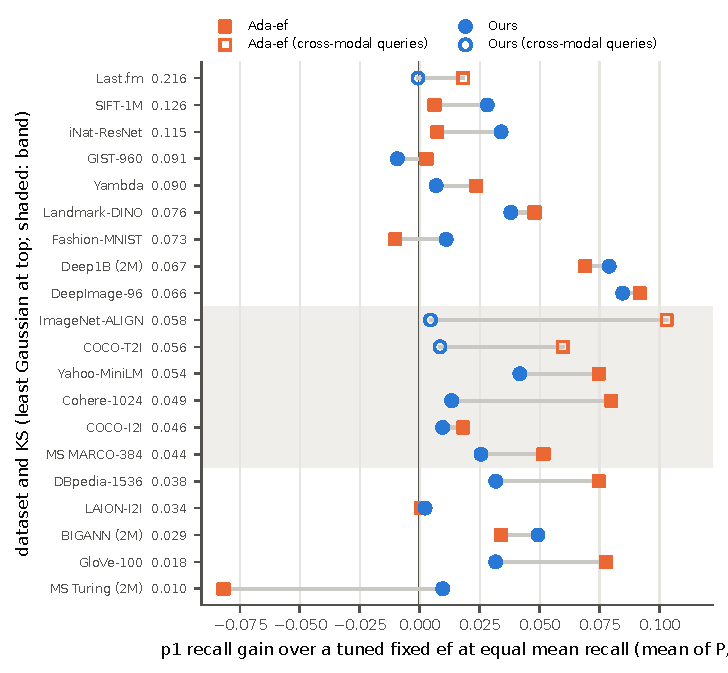
\includegraphics[width=\linewidth]{figures/fig2_p1_vs_ks.pdf}
  \caption{Tail recall (p1) gained over a fixed \ef{} at the same mean recall, for Ada-ef and
  PercEF, on 20 datasets ordered by KS (higher is less Gaussian). Ada-ef has the larger gain on 10
  of the 17 same-modality datasets and PercEF on 7: SIFT-1M, iNat-ResNet, Fashion-MNIST, Deep1B,
  LAION, BIGANN and MS Turing. KS alone does not separate the two groups. Hollow markers:
  cross-modal queries.}
  \label{fig:teaser}
\end{figure}

Graph indexes such as HNSW~\cite{malkov2020hnsw} answer a nearest-neighbor query by a best-first
walk whose breadth is set by one parameter, \ef{}. Most deployments pick one \ef{} for all
queries. That choice is wasteful in both directions: an \ef{} large enough for the hardest queries
spends work on the easy majority, and an \ef{} tuned for the average leaves the hardest queries
short of the recall the application asked for. Several recent systems therefore choose the search
effort per query, either by learning when to stop~\cite{li2020laet,chatzakis2026darth} or by
estimating, before the search, how hard the query will be~\cite{zhang2026adaef}.

Ada-ef~\cite{zhang2026adaef} takes the second route and needs no trained model.
\begin{itemize}
\item It models the similarities between a query and the database as a Gaussian, with mean and
  variance derived from the database's mean and covariance.
\item A short probe of the graph counts how many of the query's nearby points fall in the extreme
  tail of that Gaussian.
\item The count becomes a difficulty score, which maps to an \ef{}.
\end{itemize}
The method is simple and cheap. On the OpenAI and Cohere embeddings of its evaluation, it reaches
its target recall with up to 4$\times$ lower latency than learned approaches. This paper asks:
\emph{does the Gaussian model behind Ada-ef hold on the data it serves, and what decides whether
adaptive search pays off when it does not?}

At first sight, the central limit theorem seems to settle the question, since a similarity is a sum
over hundreds of dimensions. However, the theorem holds only when no small set of dimensions
dominates that sum, and whether real embeddings meet this condition has to be checked on the data.
The Ada-ef paper supports its assumption on the individual dimensions of GloVe and MS MARCO. It does
not report, dataset by dataset, how closely each query's similarities fit the Gaussian, and as far
as we can tell no other paper on nearest-neighbor search reports this either: query-hardness
measures in the literature~\cite{he2012difficulty,aumuller2019lid,wang2024steiner} either assume
such a model or avoid it. We therefore study four questions:
\begin{itemize}
\item \textbf{Q1.} How often does the Gaussian hold, and does the data type predict it?
  (\S\ref{sec:holds})
\item \textbf{Q2.} What does Ada-ef lose where the Gaussian departs? (\S\ref{sec:nongauss})
\item \textbf{Q3.} Does a nonparametric score recover that loss, and what does it give up where the
  Gaussian holds? (\S\ref{sec:nongauss}, \S\ref{sec:neargauss})
\item \textbf{Q4.} Which component carries each method's benefit and cost: the thresholds, the probe
  or the \ef{} table? (\S\ref{sec:ablation})
\end{itemize}

We measure the fit with a Kolmogorov--Smirnov (KS) statistic between each query's similarities and
the Gaussian that Ada-ef predicts. We do this on 41 datasets from ann-benchmarks, Big-ANN, VIBE and
the Ada-ef paper's own sources (Fig.~\ref{fig:survey}).

\textbf{The Gaussian departs on nine datasets.} It fits most modern text embeddings. The nine where
it departs include six learned embeddings:
\begin{itemize}
\item CNN features in DeepImage and Deep1B
\item DINO and ResNet image models
\item an audio model in Yambda
\item a factorisation model in Last.fm
\end{itemize}

\textbf{The departure hurts Ada-ef's ranking less than its size suggests.} On the eight of these
datasets whose queries share the data's modality, Ada-ef's score still ranks queries by difficulty
better than our alternative in 10 of 16 runs. It breaks down only where the departure is extreme:
\begin{itemize}
\item On Fashion-MNIST its rank correlation with the true per-query \ef{} is zero.
\item On SIFT-1M it is 0.20--0.33, and its \ef{} table uses only two values.
\item In controlled data where the hard queries move away from the bulk, its rank correlation
  changes sign.
\end{itemize}

\textbf{Ada-ef's cost is the larger problem.} Against a hindsight-tuned fixed \ef{} at the same mean
recall, Ada-ef does less work in 18 of 34 runs, but it is faster in only 6, and in none of the 16 on
the non-Gaussian datasets.

\textbf{PercEF trades ranking for cost.} To find which part of the design is responsible, we change
Ada-ef in a controlled way. PercEF reads the thresholds from the database's empirical distance
percentiles and probes 100 distances instead of 1025. It ranks queries less well than Ada-ef on most
datasets, but it is cheaper than the fixed \ef{} in 32 of 34 runs, never more than 2.5\% more
expensive, and faster in 29. To see whether the shorter probe explains this, we ran both scores at
probe lengths of 50, 100, 300 and 1025 on all 17 same-modality datasets.
\begin{itemize}
\item At equal length, the two rank queries about equally well: PercEF ranks better on 7 to 9 of the
  17 datasets.
\item PercEF still saves more latency on 14 to 15 of the datasets at every length, and more work at
  most lengths.
\item The latency gap grows with the dimension (Spearman 0.88). Ada-ef computes $q^\top\Sigma q$, a
  $d^2$ product, for every query; this alone makes it 39--85\% slower than the fixed \ef{} on the
  1536- and 2048-dimensional datasets, even with a 100-distance probe.
\end{itemize}
Where the Gaussian holds, Ada-ef's score and \ef{} table together buy larger tail gains. Learned early termination
(DARTH, LAET) buys the largest tail gains of all, at up to 2.8 times the time of a fixed \ef{}.

The overarching lesson is that \emph{a distributional assumption can fail a goodness-of-fit test
badly and still give a usable ranking; whether adaptive search pays off is decided mostly by the
fixed work it adds to every query, relative to the length of the search}. A second lesson came from
our own first evaluation. A reimplemented routine, checked only against itself, gave Ada-ef the
wrong thresholds and made the Gaussian look far worse than it is (\S\ref{sec:pitfalls}).

\textbf{Contributions.}
\begin{enumerate}
\item A per-query test of Ada-ef's Gaussian assumption on 41 public datasets. It shows where the
  assumption holds and that the data type does not predict it (\S\ref{sec:holds}).
\item An end-to-end re-evaluation of Ada-ef against a hindsight-tuned fixed \ef{}:
  \begin{itemize}
  \item matched on both mean and worst-case recall
  \item on 17 same-modality and 3 cross-modal datasets, in two calibration settings
  \item against DARTH, LAET and PiP
  \item with robustness to the target recall, $k$, the HNSW degree, the random seed and the metric
  \end{itemize}
  (\S\ref{sec:nongauss}--\S\ref{sec:analysis}).
\item PercEF, a nonparametric variant used as a controlled intervention, and an ablation that
  attributes ranking and cost to the thresholds, the probe and the \ef{} table
  (\S\ref{sec:ablation}).
\item Negative results: the KS test does not predict which score ranks better, and nothing saves work
  at $k = 10$ or adapts to cross-modal queries. Also seven pitfalls that inflate or distort measured
  savings of adaptive search (\S\ref{sec:predict}, \S\ref{sec:pitfalls}).
\end{enumerate}

% ------------------------------------------------------------------------------------------------
\section{Related Work}

\paragraph{Adaptive search in graph indexes.}
LAET~\cite{li2020laet} trains a gradient-boosted model on features gathered early in the search to
predict how much longer each query should run. DARTH~\cite{chatzakis2026darth} also terminates
early, but targets a declared recall and checks its prediction periodically during the search.
Both need a training phase with ground truth and adapt the stopping point while the search runs.
Ada-ef~\cite{zhang2026adaef} instead decides \ef{} once, after a short probe, from a statistical
model of the query's similarity distribution. It needs only the database mean and covariance and a
small calibration set, which is what makes it cheap and easy to update. PercEF keeps this design.
What we examine is the statistical model; these papers do not report its fit dataset by dataset.

\paragraph{Experimental studies of ANN search.}
Experimental surveys compare graph indexes~\cite{wang2021graphsurvey} and ANN methods across many
datasets~\cite{li2020annexperiments,aumuller2020annbenchmarks}, and show that rankings depend on the
data. We follow their approach for one design decision, the per-query \ef{}, and add something they
do not measure: the distributional assumption a method relies on. Distance distributions and their
histograms have long been used to characterise how hard a metric space is to
search~\cite{chavez2001metric}. ADSampling~\cite{gao2023adsampling} uses the concentration of
projected distances to cut distance computations. Queries drawn from a different distribution than
the data are known to hurt graph indexes~\cite{jaiswal2022ooddiskann,chen2024roargraph}. Our
cross-modal results show that they also defeat our empirical score.

\paragraph{Query and dataset hardness.}
He et al.~\cite{he2012difficulty} relate the difficulty of nearest-neighbor search to the relative
contrast between nearest and mean distances, derived under a Gaussian-type model of the data.
Aum\"uller and Ceccarello~\cite{aumuller2019lid} show that local intrinsic dimensionality and
related measures vary widely across queries in standard benchmarks and change measured performance.
Hubness~\cite{radovanovic2010hubs} describes how a few points become nearest neighbors of many
queries in high dimensions. Steiner-hardness~\cite{wang2024steiner} measures the effort a graph
index needs for a query from the index itself. These measures either describe hardness after the
fact or need the index. None asks whether the distributional model behind a cheap online score
holds, which is the question we answer with a test that runs on the raw vectors.

% ------------------------------------------------------------------------------------------------
\section{Methodology}

\subsection{Preliminaries}

Let $X \subset \mathbb{R}^d$ be the database, with vectors normalised to unit length so that
cosine similarity and Euclidean distance give the same ranking. For a query $q$ and an integer $k$,
HNSW returns $k$ candidates found by a best-first search whose candidate list holds at most \ef{}
entries. Recall@$k$ is the share of the true $k$ nearest neighbors among them. We write
$\mathrm{ef}^*(q)$ for the smallest \ef{} on a grid at which $q$ reaches the target recall $\tau$.

\paragraph{Ada-ef's score.}
Ada-ef models the distance $\delta(q,x) = 1 - q^\top x$ between $q$ and a random database vector
$x$ as
\begin{equation}
  \delta(q,x) \sim \mathcal{N}\!\left(1 - q^\top\mu,\; q^\top \Sigma q\right),
  \label{eq:clt}
\end{equation}
where $\mu$ and $\Sigma$ are the mean and covariance of $X$. It places $B = 5$ thresholds
$t_1 < \dots < t_B$ at the $\beta, 2\beta, \dots, B\beta$ quantiles of this Normal, with
$\beta = 10^{-3}$. The thresholds therefore mark the closest tenth of a percent of the database, the
next tenth, and so on. An unpruned best-first probe collects the first $L = 1025$ distances the
search meets, $P(q)$, and the score is
\begin{equation}
  s(q) = \frac{1}{|P(q)|} \sum_{p \in P(q)} w_{b(p)}, \qquad w_b = 100\, e^{-(b-1)},
  \label{eq:score}
\end{equation}
where $b(p)$ is the first bin whose threshold $p$ falls below; points beyond $t_B$ add nothing. A
query surrounded by many unusually close points scores high and is easy; a query whose probe finds
few is hard. Offline, Ada-ef scores a calibration set and groups it by rounded score. For each group
it stores the smallest \ef{} at which the group's average recall reaches $\tau$. Its paper also
floors every entry at the weighted average of these values (WAE); the released code does not. We
report both variants.

\subsection{Testing the Gaussian assumption}

Equation~\eqref{eq:clt} can be checked directly. For a query $q$ we compute the similarities
$q^\top x$ to a uniform sample of the database, and the KS statistic between their empirical
distribution and the Normal implied by~\eqref{eq:clt}:
\begin{equation}
  \KS(q) = \sup_z \left| \hat F_q(z) - \Phi\!\left(\frac{z - q^\top\mu}{\sqrt{q^\top\Sigma q}}\right) \right| .
\end{equation}
We report the mean over 200 test queries. We estimate $\mu$ and $\Sigma$ from up to $10^6$ database
vectors and $\KS(q)$ from 20{,}000. With 30 queries the estimate was as noisy as the effects we
wanted to see, so we use 200 and report a 95\% interval. The test needs only the vectors and takes a
few seconds per dataset.

\subsection{PercEF: a nonparametric control}

The thresholds in~\eqref{eq:score} are the only place where the Gaussian enters Ada-ef's score.
To test whether they are what fails, we take them from the data instead.
\begin{itemize}
\item Let $c_1,\dots,c_C$ be centroids of $X$; $C = 1$ gives the database mean.
\item For each centroid, let $t^{(c)}_b$ be the empirical $b\beta$ quantile of the squared distances
  $\lVert x - c \rVert^2$ of the database vectors assigned to it.
\item At query time we find the nearest centroid, probe the first $L = 100$ distances, and
  evaluate~\eqref{eq:score} with these thresholds and the same weights.
\end{itemize}
The thresholds thus describe what ``unusually close'' means in this particular database, whatever
the shape of its distance distribution.

Unlike Ada-ef's, these thresholds do not depend on the query. They turn Ada-ef's per-query quantiles
into fixed radii measured on the database, and the score counts how many of the probe's points fall
within them. Nothing has to be computed per query beyond the probe itself; Ada-ef needs
$q^\top\Sigma q$, a $d^2$ computation. A per-query empirical version, which would estimate each
query's own quantiles from a sample, is a natural alternative that we leave to future work.

\paragraph{Calibration.}
\begin{itemize}
\item We measure $\mathrm{ef}^*(q)$ for every calibration query.
\item We fit an isotonic regression~\cite{barlow1972isotonic} of $\mathrm{ef}^*$ on the rounded
  score, letting the fit choose the direction, and clip the result to $[k, 5000]$.
\item Optionally, we then multiply the table by one factor so that the mean recall on the
  calibration queries meets the target (\S\ref{sec:sweep}).
\end{itemize}
The search does not restart after the probe: it continues the same traversal with the chosen \ef{},
so the probe's distance computations are part of the search, not an addition to it. Our default,
fixed before the end-to-end runs, is $C = 1$ with isotonic calibration. We also ran
$C \in \{8, 50\}$ and three bucket recipes, and treat them as secondary.

The two scores differ in three ways: their thresholds, the probe length (100 against 1025) and how
the \ef{} table is built. The rank correlation we report between score and $\mathrm{ef}^*$ depends
only on the first two. We separate them by running each score with the other's probe length
(\S\ref{sec:ablation}).

\subsection{Implementation}

Both methods run inside the same HNSWlib build. Ada-ef runs through its authors' code: we call their
scoring, sketch and search routines. We made three changes:
\begin{itemize}
\item a loader that reads the database statistics from a file, so that they can be computed in one
  streaming pass
\item a replacement for the Boost normal quantile, which we check against SciPy's
\item an estimator that states Eq.~\eqref{eq:clt} in the units of our index: mean
  $2(1 - q^\top\mu)$ and variance $4\,q^\top\Sigma q$ for squared Euclidean distance on unit vectors,
  which is exact
\end{itemize}
On every dataset that fits in memory, we also built Ada-ef's estimator the original way and compared
scores on 50 queries. They are identical on 13 of the 17 datasets. On SIFT-1M, BIGANN, DBpedia and
COCO-I2I they differ on some queries, by at most 0.39 in score. Our score is computed inside the same traversal, with the same
memory prefetching as HNSWlib's own search loop. All searches run on one thread.

% ------------------------------------------------------------------------------------------------
\section{Experiments}

\subsection{Setup}

\paragraph{Datasets.}
We benchmark 20 datasets end to end (Table~\ref{tab:datasets}):
\begin{itemize}
\item the four in the Ada-ef paper that we could obtain: GloVe-100, DeepImage-96, Cohere-1024 and
  LAION-I2I, the last two as subsets that fit in 62\,GB of memory
\item a MiniLM-384 stand-in for its MS MARCO set
\item standard ann-benchmarks sets~\cite{aumuller2020annbenchmarks}
\item 2M-vector prefixes of three Big-ANN sets~\cite{simhadri2022bigann}; the benchmark builds its own
  subsets the same way
\item four VIBE sets~\cite{jaasaari2025vibe}
\item Yambda audio embeddings~\cite{ploshkin2025yambda}
\end{itemize}
Three of the datasets have queries from a different modality than the database (text against images,
users against songs).

\paragraph{Protocol.}
We follow the Ada-ef paper:
\begin{itemize}
\item HNSW with $M = 16$ and $\mathit{ef}_{\mathrm{construction}} = 500$
\item $k = 1000$ for the MS MARCO, Cohere and LAION sets and $k = 100$ otherwise
\item target recall $\tau = 0.95$, and \ef{} capped at 5000
\end{itemize}
Both methods always calibrate on the same set, in two settings: \emph{P}, 200 database vectors as in
the Ada-ef paper, and \emph{R}, up to 2000 held-out real queries. Test queries are disjoint from
both.

\paragraph{Metrics.}
Ada-ef's stated aims are to meet a declared target recall while avoiding both under- and
over-searching~\cite{zhang2026adaef}. We use the same recall statistics its evaluation reports:
\begin{itemize}
\item mean recall
\item the 1st and 5th percentiles of per-query recall (p1, p5), which ``capture performance on the
  hardest queries'' and so show under-searching~\cite[\S 7.2]{zhang2026adaef}
\end{itemize}
We measure cost in three ways:
\begin{itemize}
\item latency per query, as the Ada-ef paper does
\item distance computations (DC), including every probe, which the Ada-ef paper does not report and
  which serve as a hardware-independent measure of cost
\item offline time and memory
\end{itemize}
We count DC as HNSWlib does, as every neighbor-list entry a search examines, visited or not. All
methods run in HNSWlib are counted the same way.

\paragraph{The fixed-\ef{} reference.}
We run HNSW at a grid of fixed \ef{} values and, for each method, interpolate the fixed \ef{} that
reaches the same mean recall. This is the best fixed \ef{} anyone could choose in hindsight; no
deployment can pick it in advance, so beating it is a demanding test. The Ada-ef paper instead sweeps
the fixed \ef{} upward until mean recall reaches 0.99 and compares the curves, so it does not match
the two at equal mean recall. We interpolate in $\log(1 - \text{recall})$ against $\log$ cost.
Interpolating linearly overstates the fixed \ef{}'s cost by 11\% on average in a leave-one-out test
on our grids (\S\ref{sec:pitfalls}), which would flatter every adaptive method.

\begin{table}[t]
  \caption{Datasets, sorted by KS (200 queries). $\rho$: rank correlation between each score and
  the true per-query $\mathrm{ef}^*$ on the calibration set, settings P / R; the larger magnitude
  ranks queries better. A dash: the score is constant on the calibration queries.}
  \label{tab:datasets}
  \centering\footnotesize
  \resizebox{\linewidth}{!}{\begin{tabular}{lllrrrrrrrrr}
\toprule
dataset & source & in Ada-ef paper & corpus & dim & K & test queries & KS & rho Ada-ef P & rho ours P & rho Ada-ef R & rho ours R \\
\midrule
MS Turing (2M) & Big-ANN & no & 2,000,000 & 100 & 100 & 10000 & 0.010 & -0.81 & -0.35 & -0.79 & -0.40 \\
GloVe-100 & ann-benchmarks & yes & 1,183,514 & 100 & 100 & 8000 & 0.018 & -0.87 & -0.61 & -0.88 & -0.61 \\
BIGANN (2M) & Big-ANN & no & 2,000,000 & 128 & 100 & 8000 & 0.029 & -0.62 & -0.74 & -0.61 & -0.74 \\
LAION-I2I & LAION, shards 0-19 & yes (subset) & 19,639,187 & 512 & 1000 & 10000 & 0.034 & -0.39 & -0.56 & -0.40 & -0.53 \\
DBpedia-1536 & DBpedia, OpenAI embeddings & no & 990,000 & 1536 & 100 & 8000 & 0.038 & -0.63 & -0.38 & -0.66 & -0.54 \\
MS MARCO-384 & MS MARCO (MiniLM) & stand-in & 8,841,823 & 384 & 1000 & 6980 & 0.044 & -0.62 & -0.53 & -0.64 & -0.53 \\
COCO-I2I & ann-benchmarks & no & 113,287 & 512 & 100 & 8000 & 0.046 & -0.38 & -0.39 & -0.40 & -0.36 \\
Cohere-1024 & Cohere, files 00-04 & yes (subset) & 9,511,868 & 1024 & 1000 & 1174 & 0.049 & -0.50 & -0.40 & -0.73 & -0.52 \\
Yahoo-MiniLM & VIBE & no & 677,305 & 384 & 100 & 700 & 0.054 & -0.58 & -0.54 & -0.56 & -0.68 \\
COCO-T2I & ann-benchmarks & no & 113,287 & 512 & 100 & 8000 & 0.056 & -0.39 & -0.38 & -0.57 & -- \\
ImageNet-ALIGN & VIBE & no & 1,281,167 & 640 & 100 & 1000 & 0.058 & -0.22 & -0.23 & -0.24 & -- \\
DeepImage-96 & ann-benchmarks & yes & 9,990,000 & 96 & 100 & 8000 & 0.066 & -0.76 & -0.63 & -0.75 & -0.62 \\
Deep1B (2M) & Big-ANN & no & 2,000,000 & 96 & 100 & 8000 & 0.067 & -0.77 & -0.64 & -0.76 & -0.67 \\
Fashion-MNIST & ann-benchmarks & no & 60,000 & 784 & 100 & 8000 & 0.073 & +0.05 & -0.22 & -0.00 & -0.29 \\
Landmark-DINO & VIBE & no & 760,757 & 768 & 100 & 700 & 0.076 & -0.70 & -0.61 & -0.64 & -0.55 \\
Yambda & Yambda & no & 7,709,749 & 128 & 100 & 10000 & 0.090 & -0.38 & -0.41 & -0.45 & -0.43 \\
GIST-960 & ann-benchmarks & no & 1,000,000 & 960 & 100 & 700 & 0.091 & -0.63 & -0.46 & -0.62 & -0.23 \\
iNat-ResNet & VIBE & no & 499,000 & 2048 & 100 & 700 & 0.115 & -0.49 & -0.46 & -0.36 & -0.46 \\
SIFT-1M & ann-benchmarks & no & 1,000,000 & 128 & 100 & 8000 & 0.126 & -0.20 & -0.33 & -0.33 & -0.45 \\
Last.fm & ann-benchmarks & no & 292,385 & 65 & 100 & 10000 & 0.216 & -0.09 & +0.23 & -0.00 & -- \\
\bottomrule
\end{tabular}
}
\end{table}

\subsection{How often does the assumption hold?}\label{sec:holds}

Figure~\ref{fig:survey} shows KS for all 41 datasets. Most lie below 0.044. They are mostly text and
text-image embeddings (OpenAI, Cohere, MiniLM, Nomic, CLIP and others), but word vectors, LLM
attention keys and SIFT-1B are among them too. Nine lie at or above 0.066: SIFT-1M, GIST,
Fashion-MNIST, DeepImage, Deep1B, iNaturalist ResNet, Landmark DINO, Yambda and Last.fm.

We fixed the band 0.044--0.066 from our first six datasets and use it throughout to group the
results. It is a grouping, not a dividing line between the two methods (\S\ref{sec:predict}).

Datasets built from the same kind of data land on different sides: SIFT-1M at 0.126 and SIFT-1B at
0.029, Fashion-MNIST at 0.073 and MNIST at 0.037. So the assumption has to be checked on the data
itself.

\begin{figure}[t]
  \centering
  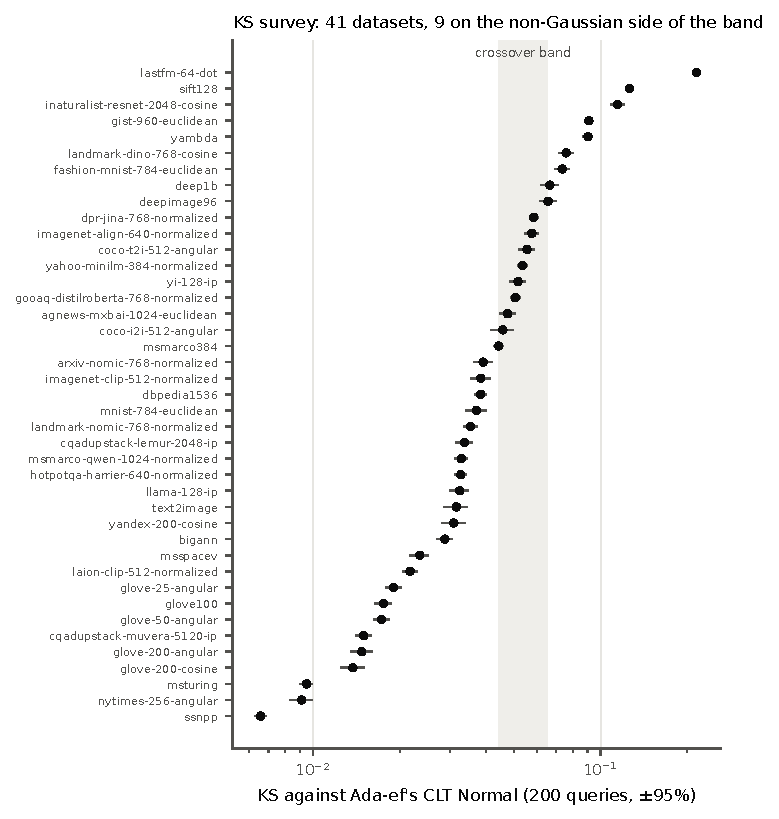
\includegraphics[width=0.92\linewidth]{figures/fig1_ks_survey.pdf}
  \caption{KS between each query's similarities and Ada-ef's Gaussian, mean over 200 queries with
  95\% interval, for 41 public datasets. Shaded: the band 0.044--0.066 we use to group results.
  GloVe-200 appears twice, from ann-benchmarks and from VIBE.}
  \label{fig:survey}
\end{figure}

\subsection{Comparison on non-Gaussian datasets}\label{sec:nongauss}

Table~\ref{tab:counts} summarises every run against the fixed-\ef{} reference, and
Fig.~\ref{fig:cost} shows where each method sits relative to the fixed-\ef{} curve.

\paragraph{Ranking.}
On the eight same-modality datasets above the band (16 runs), Ada-ef's score has the larger rank
correlation with $\mathrm{ef}^*$ in 10. On DeepImage, Deep1B and Landmark-DINO it ranks queries well,
with $|\rho|$ = 0.64--0.77 against PercEF's 0.55--0.67, even though KS is 0.066--0.076 there. Its
score breaks down where the departure is extreme:
\begin{itemize}
\item On Fashion-MNIST it is uncorrelated with $\mathrm{ef}^*$ ($\rho = +0.05$ and $0.00$) and gives
  every calibration point the same \ef{} in setting P.
\item On SIFT-1M its correlation is 0.20 and 0.33, against PercEF's 0.33 and 0.45, and its table uses
  only two distinct \ef{} values.
\end{itemize}
GIST (KS 0.091) is the opposite case: Ada-ef ranks clearly better there (0.62 against 0.46 and 0.23).

\paragraph{Cost.}
Cost separates the methods more clearly than ranking does.
\begin{itemize}
\item PercEF is cheaper than the fixed \ef{} in 14 of the 16 runs. The two exceptions are small:
  DeepImage P costs 2.5\% more and GIST R 0.8\% more.
\item Ada-ef is cheaper in 9 of the 16 runs and faster in none. Its probe makes it 4--93\% slower
  than the fixed \ef{} at the same recall.
\item Ada-ef's worst run is Fashion-MNIST, at 24.8\% more work. There most queries reach the target
  at the smallest \ef{}, so a long probe is pure overhead.
\end{itemize}

\paragraph{Tail recall.}
Both methods usually keep or raise the tail: p1 is at or above the fixed \ef{}'s in 13 of 16 runs
for each.
\begin{itemize}
\item Ada-ef's p1 gains are larger on DeepImage (0.090 and 0.094 against 0.081 and 0.088),
  Landmark-DINO and Yambda.
\item PercEF's are larger on SIFT-1M (0.028--0.029 against 0.004--0.008), iNaturalist
  (0.030--0.038 against 0.004--0.011), Fashion-MNIST and Deep1B.
\end{itemize}

\paragraph{Matched on p1.}
Matching the fixed \ef{} on mean recall credits each method with the work it saves but not with the
tail it buys. Matched instead on p1, that is, against the cheapest fixed \ef{} that serves the worst
1\% of queries as well:
\begin{itemize}
\item PercEF is faster in 14 of the 16 runs, by a median of 16\%.
\item Ada-ef is faster in 4.
\end{itemize}

\begin{table}[t]
  \caption{Runs in which each method is cheaper than the fixed \ef{} at the same mean recall (DC),
  faster (latency, every run timed), and has at least its p1 tail recall; and runs in which it is
  faster than the fixed \ef{} with the same p1 (p1-matched). Same modality unless marked. Worst:
  the largest extra cost (negative: more work than the fixed \ef{}).}
  \label{tab:counts}
  \centering\footnotesize\setlength{\tabcolsep}{3.5pt}
  \begin{tabular}{llrrrrr}
    \toprule
    & & \multicolumn{4}{c}{same mean recall} & p1-matched \\
    \cmidrule(lr){3-6}\cmidrule(lr){7-7}
    Datasets & Method & Cheaper & Worst & Faster & p1 $\geq$ & Faster \\
    \midrule
    All (34 runs)        & Ours        & 32/34 & $-$2.5\%  & 29/34 & 31/34 & 32/34 \\
                         & Ada-ef      & 18/34 & $-$24.8\% &  6/34 & 29/34 & 13/34 \\
                         & Ada-ef WAE  & 24/34 & $-$24.8\% &  8/34 & 29/34 & 16/34 \\
    \midrule
    KS $\geq$ 0.066 (16) & Ours        & 14/16 & $-$2.5\%  & 11/16 & 13/16 & 14/16 \\
                         & Ada-ef      &  9/16 & $-$24.8\% &  0/16 & 13/16 &  4/16 \\
    Band (8)             & Ours        &   8/8 & $+$3.4\%  &   8/8 &   8/8 &   8/8 \\
                         & Ada-ef      &   3/8 & $-$4.5\%  &   3/8 &   8/8 &   6/8 \\
    KS $<$ 0.044 (10)    & Ours        & 10/10 & $+$2.4\%  & 10/10 & 10/10 & 10/10 \\
                         & Ada-ef      &  6/10 & $-$15.2\% &  3/10 &  8/10 &  3/10 \\
                         & Ada-ef WAE  &  9/10 & $-$4.4\%  &  5/10 &  7/10 &  4/10 \\
    \midrule
    Cross-modal (6)      & Ours        &   2/6 & $-$1.0\%  &   3/6 &   5/6 &   5/6 \\
                         & Ada-ef      &   1/6 & $-$20.2\% &   0/6 &   6/6 &   1/6 \\
    \bottomrule
  \end{tabular}
\end{table}

\begin{figure*}[t]
  \centering
  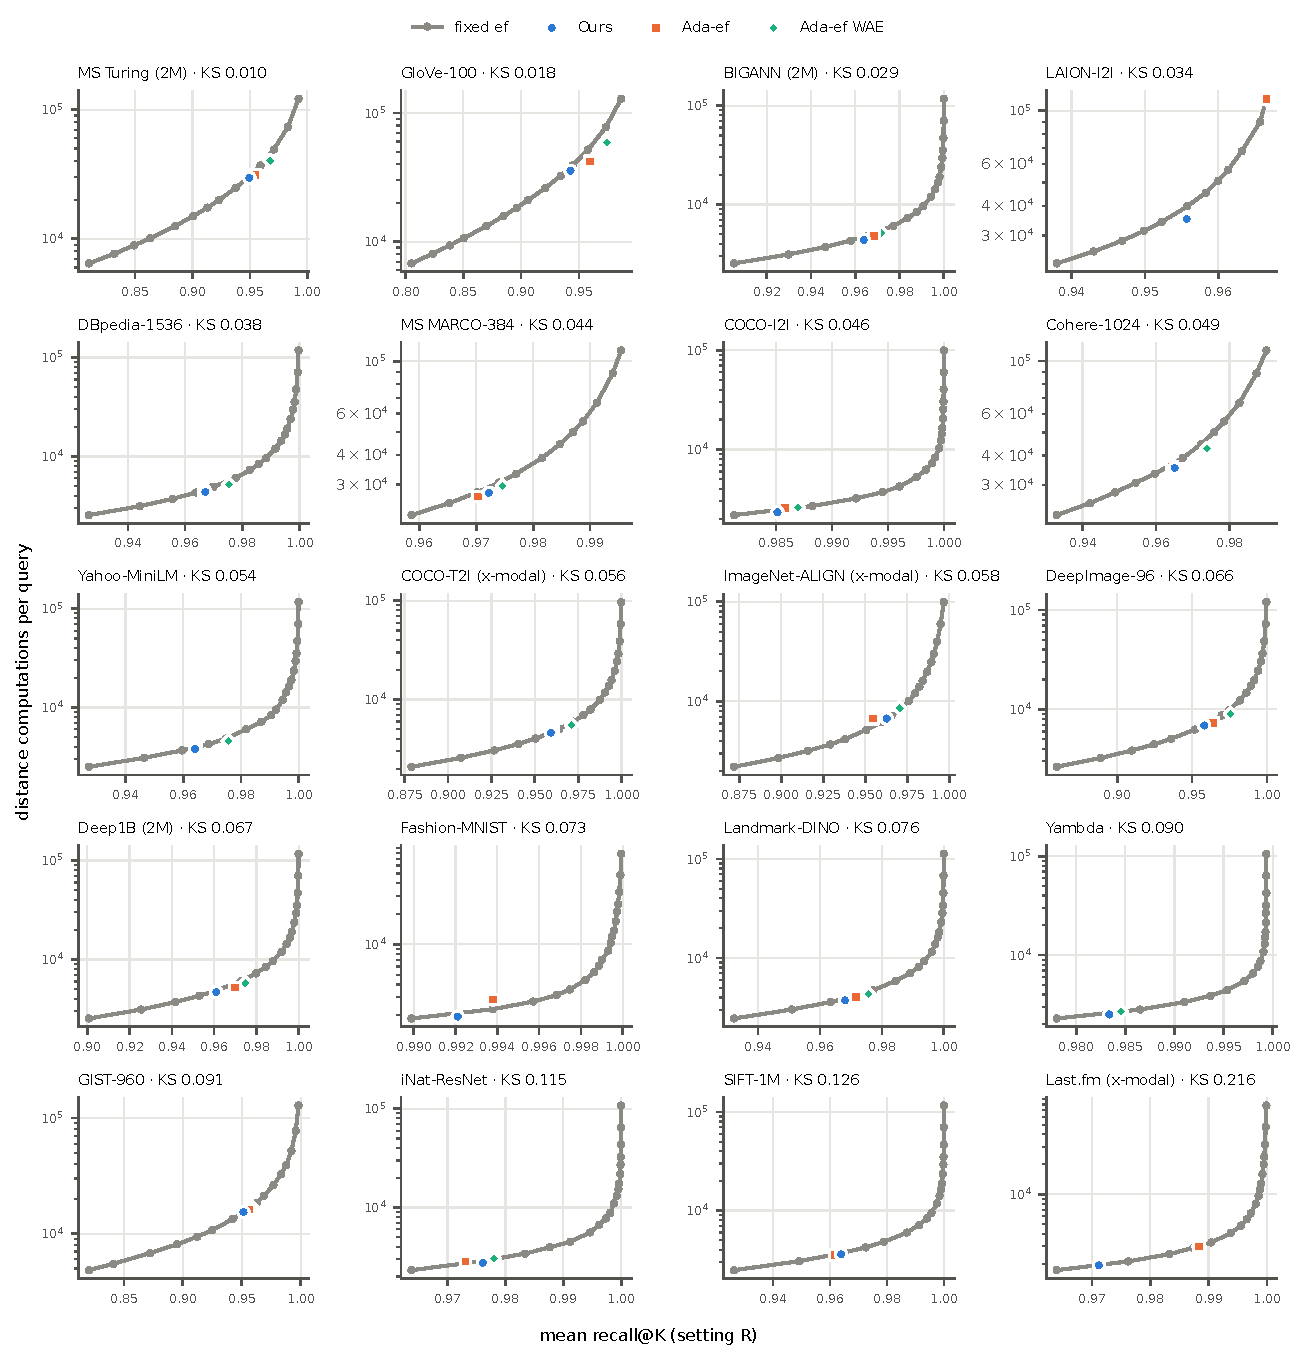
\includegraphics[width=0.95\textwidth]{figures/fig3_cost_vs_recall.pdf}
  \caption{Distance computations per query against mean recall, setting R. Grey: HNSW with fixed
  \ef{}. Points below the curve reach the same recall with less work. Panels are ordered by KS, from
  near-Gaussian (top left) to non-Gaussian (bottom right).}
  \label{fig:cost}
\end{figure*}

\subsection{Comparison on near-Gaussian datasets}\label{sec:neargauss}

In and below the band, Ada-ef's model fits and its score shows it. It ranks queries better than
PercEF in 12 of the 18 runs, by the widest margins on:
\begin{itemize}
\item MS Turing: 0.79--0.81 against 0.35--0.40
\item GloVe: 0.87--0.88 against 0.61
\item DBpedia, MS MARCO and Cohere
\end{itemize}
Its tail gains are larger too: p1 rises by 0.071--0.084 on GloVe, 0.048--0.056 on MS MARCO and
0.060--0.100 on Cohere, against PercEF's 0.029--0.034, 0.025--0.026 and 0.009--0.017.

With its WAE floor, Ada-ef is also much cheaper than the fixed \ef{} on GloVe (26--27\%) and MS
Turing (6--11\%), more than PercEF's 5--6\% and 2--3\%. On GloVe it is faster in wall-clock time by
21\%.

PercEF, in turn, is cheaper and faster than the fixed \ef{} in all 18 runs, never lowers its tail,
and is faster than its own p1-matched fixed \ef{} in all 18. Ada-ef as shipped is cheaper in 9 and
faster in 6.

The near-Gaussian side is therefore a real trade-off. Ada-ef is the better choice where searches are
long and the worst-served queries matter most; PercEF is the better choice where a predictable cost
does.

Two datasets on this side behave differently:
\begin{itemize}
\item \textbf{BIGANN} (SIFT-1B, KS 0.029) and \textbf{LAION}: our score ranks queries better
  (0.74 against 0.61--0.62 on BIGANN; 0.53--0.56 against 0.39--0.40 on LAION) and saves the most work
  of any method (7--8\% and 11\%).
\item \textbf{MS Turing} (KS 0.010): Ada-ef ranks best, yet its tail is worse than the fixed \ef{}'s
  (p1 $-$0.086 and $-$0.078). Its group-average table under-provisions some score groups; the WAE
  floor narrows the loss to $-$0.067 and $-$0.006.
\end{itemize}

\subsection{Analysis}\label{sec:analysis}

\paragraph{Does KS predict the better score?}\label{sec:predict}
We had set the band from our first six datasets. Before running each of the other fourteen, we wrote
down which score would rank its queries better. Against the corrected Ada-ef (\S\ref{sec:pitfalls}),
these predictions held on only 4 of the 9 datasets for which we made a definite prediction.

Across the 17 same-modality datasets, KS correlates with Ada-ef's rank correlation at only $-0.43$
(Spearman). Datasets with moderate KS divide in both directions:
\begin{itemize}
\item DeepImage, Deep1B, Landmark-DINO and GIST, where Ada-ef ranks well
\item BIGANN and LAION, below the band, where PercEF ranks better
\end{itemize}
KS therefore tells whether Ada-ef's model is accurate, not whether its ranking is usable. It is not
a rule for choosing between the two scores. Nor does KS single out the collapses: SIFT-1M and
Fashion-MNIST are non-Gaussian, but so are DeepImage and GIST, where Ada-ef ranks well. A cheap
check helps in practice. Ada-ef's calibration already scores a few hundred points, and when its
table maps them to one or two \ef{} values (SIFT-1M, Fashion-MNIST, and Yambda in setting P), the
score cannot separate queries at run time, whatever its correlation.

\paragraph{Which component carries the benefit?}\label{sec:ablation}
Ada-ef's score has three parts: Gaussian thresholds, a 1025-distance probe and a group-average \ef{}
table. PercEF changes the first two, so we ran each score with the other's probe length
(Table~\ref{tab:ablation}).

\begin{itemize}
\item \textbf{Ranking.} At equal probe length, the empirical thresholds rank queries better on
  SIFT-1M and BIGANN, by 0.07 to 0.11. The Gaussian thresholds rank better on Deep1B, DeepImage and
  MS Turing at both lengths, and on GloVe at 1025 distances. The two tie on GloVe at 100. So the
  thresholds matter, but in Ada-ef's favour on most of these datasets.
\item \textbf{Probe length and the near-Gaussian edge.} Ada-ef's edge on GloVe and MS Turing comes
  from its long probe. Cut to 100 distances, its rank correlation falls from 0.88 to 0.62 on GloVe
  and from 0.79 to 0.43 on MS Turing.
\item \textbf{Probe length and cost.} The probe explains part of the cost difference, not all of
  it. We ran both scores at 50, 100, 300 and 1025 distances on all 17 same-modality datasets
  (Table~\ref{tab:probes}).
  \begin{itemize}
  \item At equal length, PercEF saves more latency than Ada-ef on 14--15 datasets and more work on
    10--16. Its rank correlation is higher on only 7--9.
  \item Each method at its own best probe length: PercEF is faster than the fixed \ef{} on 15 of the
    17 datasets, Ada-ef on 4, and Ada-ef with the WAE floor on 8.
  \item The latency gap at equal length correlates with the dimension at 0.88 (Spearman, 16
    datasets). Ada-ef computes $q^\top\Sigma q$ for every query, a $d^2$ product: with a 100-distance
    probe it is still 39\% slower than the fixed \ef{} on DBpedia ($d = 1536$) and 85\% on iNaturalist
    ($d = 2048$), but within 3\% on all six datasets with $d \le 128$.
  \end{itemize}
  So on low-dimensional data, Ada-ef with a short probe costs about what PercEF does. On
  high-dimensional data, its per-query variance does not.
\item \textbf{Tail.} Better ranking alone does not buy Ada-ef's tail. With 1025 distances, PercEF's
  p1 gain on GloVe stays at 0.028 against Ada-ef's 0.082. With Ada-ef's own table (each score group
  gets the smallest \ef{} at which the group's average recall reaches the target), PercEF's p1 gain on
  GloVe is 0.031. Ada-ef's tail on these datasets needs its score and its table together. On the
  non-Gaussian sets the same table lowers PercEF's tail slightly (DeepImage 0.088 to 0.073), so we
  keep PercEF's own calibration.
\end{itemize}

\begin{table}[t]
  \caption{Rank correlation $|\rho|$ between each score and $\mathrm{ef}^*$ when both scores use
  each probe length $L$ (setting R). Bold: the better score at that probe length.}
  \label{tab:ablation}
  \centering\footnotesize
  \begin{tabular}{lrrrrr}
    \toprule
    & & \multicolumn{2}{c}{Ada-ef} & \multicolumn{2}{c}{PercEF} \\
    Dataset & KS & $L$=1025 & $L$=100 & $L$=100 & $L$=1025 \\
    \midrule
    SIFT-1M   & 0.126 & 0.33 & 0.35 & \textbf{0.45} & \textbf{0.40} \\
    Deep1B    & 0.067 & \textbf{0.76} & \textbf{0.74} & 0.67 & 0.63 \\
    DeepImage & 0.066 & \textbf{0.75} & \textbf{0.72} & 0.62 & 0.59 \\
    SIFT-1B   & 0.029 & 0.61 & 0.65 & \textbf{0.74} & \textbf{0.72} \\
    GloVe     & 0.018 & \textbf{0.88} & 0.62 & 0.61 & 0.76 \\
    MS Turing & 0.010 & \textbf{0.79} & \textbf{0.43} & 0.40 & 0.58 \\
    \bottomrule
  \end{tabular}
\end{table}

\begin{table}[t]
  \caption{Probe-length sweep, both scores at each probe length $L$, 17 same-modality datasets,
  setting R: datasets on which PercEF is ahead of Ada-ef (as shipped) at the same $L$. Savings are
  against the tuned fixed \ef{} at the same mean recall; a dataset counts where both have a value.
  Bottom: each method at its own best $L$.}
  \label{tab:probes}
  \centering\footnotesize\setlength{\tabcolsep}{3.5pt}
  \begin{tabular}{lrrrr}
    \toprule
    $L$ & Higher $|\rho|$ & More work saved & More time saved & Larger p1 gain \\
    \midrule
    50   &  8/17 & 16/17 & 15/17 & 10/17 \\
    100  &  9/17 & 12/16 & 14/16 &  8/16 \\
    300  &  8/17 & 12/16 & 14/16 &  7/16 \\
    1025 &  7/17 & 10/17 & 15/17 &  6/17 \\
    \midrule
    best $L$ each & -- & 11/17 & 15/17 & -- \\
    \bottomrule
  \end{tabular}
\end{table}

\paragraph{Latency and offline cost.}\label{sec:latency}
Ada-ef's wall-clock cost depends on how long the searches are. Its probe is a fixed 1025 distances.
\begin{itemize}
\item \textbf{Long searches.} On searches of several milliseconds the probe is a small share, and
  there Ada-ef can be faster than the fixed \ef{} at the same recall: the WAE variant by 21\% on
  GloVe and 9\% on MS Turing R; the shipped variant by 6--12\% on Cohere.
\item \textbf{Short searches.} The probe dominates. Ada-ef is 4--93\% slower than the fixed \ef{} on
  the non-Gaussian datasets, and 32--115\% slower on Last.fm, where a whole search takes 0.13\,ms.
\item \textbf{PercEF.} At the same mean recall, PercEF is faster than the fixed \ef{} in 29 of 34
  runs: all 18 in or below the band, by 1\% to 16\%, and 11 of the 16 non-Gaussian runs. In the other
  5 it is slower by at most 2.5\%, except on DeepImage (8.3\%). Against Ada-ef directly, PercEF is
  faster in 31 of 34 runs.
\end{itemize}

\paragraph{Why time saved lags work saved.}
Not every distance computation costs the same. Under a plain fixed \ef{}, compare queries with the
same distance count (Table~\ref{tab:querycost}):
\begin{itemize}
\item the queries PercEF classifies as hard (top 20\% of its \ef{}) take a median 8\% more time
\item the queries it calls easy take 11\% less
\end{itemize}
This is probably because hard queries wander through less cached parts of the graph. PercEF moves
work from easy queries to hard ones, so it saves cheap distance computations and spends dearer ones.
Its time per distance computation is a median 1\% above the fixed \ef{}'s: 0.3\% above the band and
2.5\% in or below it.

\paragraph{Offline cost.}
Both methods need seconds for their statistics. Calibration time is dominated by two steps:
\begin{itemize}
\item measuring $\mathrm{ef}^*$ for PercEF, up to 257\,s on MS Turing
\item Ada-ef's per-group search, 183\,s on MS Turing and up to 370\,s on GloVe
\end{itemize}
Ada-ef keeps a $d \times d$ covariance, up to 9.4\,MB at $d = 1536$. Ours keeps five thresholds, the
centroid and the table: a few kilobytes.

\paragraph{Other targets and $k$.}\label{sec:sweep}
All results so far use the Ada-ef paper's protocol ($\tau = 0.95$, $k = 100$ or $1000$). We repeated
the comparison at $\tau = 0.90$ and $0.99$ and at $k = 10$, in both settings
(Table~\ref{tab:sweep}), on six datasets:
\begin{itemize}
\item four above the band: DeepImage, Deep1B, SIFT-1M and Landmark-DINO
\item two below it: GloVe and MS Turing
\end{itemize}

At both other targets, the picture of \S\ref{sec:nongauss} holds:
\begin{itemize}
\item Above the band, PercEF does less work than the tuned fixed \ef{} in 7 and 6 of the 8 runs,
  never more than 2.2\% extra. It never lowers p1 and is faster than the p1-matched fixed \ef{} in all
  8, by a median of 18--19\%.
\item Ada-ef does less work in 5 and 8 of the 8 runs, but it is faster than the fixed \ef{} at the
  same recall in at most 1.
\item Below the band, PercEF wins on every count in all 4 runs at both targets.
\item At $\tau = 0.99$, Ada-ef with the WAE floor is cheaper than the fixed \ef{} in all 8 runs
  above the band.
\end{itemize}

\paragraph{Weakness 1: PercEF's mean recall lands further from the target.}
Our table maps a score to the average $\mathrm{ef}^*$ of similar calibration queries and never checks
the mean recall that results; Ada-ef's table is built to meet the target. Every comparison above is
made at the method's own recall, so the counts are not affected. The gap closes with one offline
step: we multiply the whole table by a single factor, the smallest whose mean recall on the
calibration queries reaches $\tau$. It is found by bisection, and nothing changes per query. With it,
PercEF's mean recall lands within 0.01 of the target:
\begin{itemize}
\item above the band: in 7 of the 8 runs at $\tau = 0.95$ (Ada-ef: 2), and in all 8 at
  $\tau = 0.99$ (Ada-ef: 8)
\item below the band: in 3 of the 4 runs at each target
\end{itemize}
Its advantage over the fixed \ef{} survives. Above the band it still does less work in 6 and 7 of
the 8 runs, at most 4.5\% extra, and is faster than the p1-matched fixed \ef{} in all 8, by a median
of 17--19\%.

\paragraph{Weakness 2: at $k = 10$ neither method saves work.}
\begin{itemize}
\item PercEF needs up to 19\% more than the tuned fixed \ef{} above the band, cheaper in 0 of 8 runs.
\item Ada-ef needs up to 69\% more, and is cheaper in 1 of 12 runs.
\end{itemize}
The probe is not the cause: with a 30-distance probe, PercEF is still cheaper in none of the 8 runs.
A likely reason is that recall moves in steps of 0.1 per query, so each query's $\mathrm{ef}^*$ is
too coarse for any score to predict. We leave small $k$ open. For the same reason the p1-matched
comparison is not meaningful at $k = 10$.

\begin{table}[t]
  \caption{Robustness sweep, six datasets, settings P and R. Counts against the tuned fixed \ef{}:
  less work at the same mean recall, p1 at least the fixed \ef{}'s, and faster than the p1-matched
  fixed \ef{} (median time saving). Above: 4 datasets above the band (8 runs); below: 2 below it (4).}
  \label{tab:sweep}
  \centering\footnotesize\setlength{\tabcolsep}{3.5pt}
  \begin{tabular}{lllrrr}
    \toprule
    $\tau$, $k$ & Data & Method & Less work & p1 $\geq$ & p1-matched faster \\
    \midrule
    0.90, 100 & above & Ours   & 7/8 & 8/8 & 8/8 (18\%) \\
              &       & Ada-ef & 5/8 & 6/8 & 3/8 \\
              & below & Ours   & 4/4 & 4/4 & 4/4 (11\%) \\
              &       & Ada-ef & 0/4 & 2/4 & 2/4 \\
    \midrule
    0.95, 100 & above & Ours   & 7/8 & 8/8 & 8/8 (24\%) \\
              &       & Ada-ef & 7/8 & 8/8 & 4/8 \\
              & below & Ours   & 4/4 & 4/4 & 4/4 (10\%) \\
              &       & Ada-ef & 2/4 & 2/4 & 2/4 \\
    \midrule
    0.99, 100 & above & Ours   & 6/8 & 8/8 & 8/8 (19\%) \\
              &       & Ada-ef & 8/8 & 6/8 & 4/8 \\
              & below & Ours   & 4/4 & 4/4 & 4/4 (11\%) \\
              &       & Ada-ef & 3/4 & 2/4 & 2/4 \\
    \midrule
    0.95, 10  & above & Ours   & 0/8 & 8/8 & -- \\
              &       & Ada-ef & 0/8 & 6/8 & -- \\
              & below & Ours   & 2/4 & 3/4 & -- \\
              &       & Ada-ef & 1/4 & 3/4 & -- \\
    \bottomrule
  \end{tabular}
\end{table}

\paragraph{Index degree, seeds and metric.}
\begin{itemize}
\item \textbf{HNSW degree.} At $M = 8$ and $M = 32$ on SIFT-1M, Deep1B, GloVe and MS Turing, PercEF
  is cheaper than the fixed \ef{} in 14 of 16 runs and Ada-ef in 11. Ada-ef is faster in 4 of 16 and
  PercEF in 8. Ada-ef keeps its edge in work on GloVe, and PercEF on SIFT-1M and MS Turing, as at
  $M = 16$.
\item \textbf{Seeds.} With three random seeds for the calibration and test split on SIFT-1M,
  DeepImage, GloVe and MS Turing, the ordering of the two methods is the same in every seed. PercEF's
  saving keeps its sign except on DeepImage, where it ranges from $-$6.1\% to $+$2.7\%.
\item \textbf{Metric.} On raw, unnormalised vectors with Euclidean distance (SIFT-1M, GIST,
  Fashion-MNIST, BIGANN, Deep1B, MS Turing), PercEF is cheaper than the fixed \ef{} in 11 of 12 runs,
  by up to 7.7\% (BIGANN). Ada-ef's estimator assumes unit vectors, so it does not apply.
\end{itemize}

\paragraph{Learned methods and PiP.}
DARTH~\cite{chatzakis2026darth} stops each search when a gradient-boosted model, fed with features
of the search so far, predicts that the target recall has been reached. LAET~\cite{li2020laet}
predicts once, after a fixed number of distance computations, how many the query needs in total.

We ran both through DARTH's authors' FAISS fork, which contains LAET's search. It is unchanged apart
from a build path and a data loader. We ran on seven datasets: GloVe, MS Turing and DBpedia below
the band, and DeepImage, Deep1B, Landmark-DINO and SIFT-1M above it.
\begin{itemize}
\item They use the same test queries and ground truth, $M = 16$,
  $\mathit{ef}_{\mathrm{construction}} = 500$ and one thread.
\item They are trained on 1,500 calibration queries (DARTH's paper uses 10,000) and tuned on the
  other 500: DARTH's prediction intervals as in its authors' scripts, and LAET's prediction point and
  multiplier so that validation recall meets the target.
\item Each method is compared with a fixed \ef{} of its own library, because the two HNSW
  implementations build different graphs, time queries differently and count work differently.
  FAISS counts only the distances it computes: at the same recall its fixed \ef{} reports 0.59 to 0.71
  times HNSWlib's count on these datasets (Table~\ref{tab:darth}).
\end{itemize}

DARTH has the best p1 gain on four of the seven datasets, Ada-ef on two and LAET on one. Both learned
methods pay for their tail gains in time:
\begin{itemize}
\item They are slower than their fixed \ef{} on every dataset but one (LAET on GloVe, 1.3\% faster),
  by up to 2.8 times where a search takes about a millisecond and the model calls dominate.
\item They do less work than the fixed \ef{} only on the two long-search datasets, GloVe and MS
  Turing, by 7--18\%, and 3--20\% more on the other five.
\item Each needs 2 to 10 minutes of training and tuning per dataset and gigabytes of search traces.
\end{itemize}
On seven more datasets (BIGANN, COCO-I2I, Fashion-MNIST, GIST, iNaturalist, Yahoo-MiniLM and Yambda)
we ran DARTH alone. It is 53--85\% slower than its fixed \ef{} on the three where the two can be
matched. On the other four, its mean recall stays below that of FAISS's smallest fixed \ef{}.

Corrected, Ada-ef also does less work than the fixed \ef{} on all seven datasets in
Table~\ref{tab:darth}, and more savings than PercEF on four of them. But it is faster only on GloVe
and MS Turing. PercEF is faster than its fixed \ef{} on five of the seven, and at most 8.3\% slower
on the others.

PiP (patience in proximity), the early-stopping rule that Ada-ef's code base ships, behaves
differently:
\begin{itemize}
\item At its paper's setting it falls well short of the target (mean recall 0.79--0.81 on SIFT-1M and
  Deep1B).
\item Tuned on our calibration queries, it saves between $-$1.4\% and $+$1.7\% of the work.
\item Its implementation copies the result list at every step, so we compare it on work only.
\end{itemize}

\begin{table}[t]
  \caption{Learned methods (DARTH, LAET; FAISS), Ada-ef (as shipped) and PercEF (HNSWlib) against a
  tuned fixed \ef{} of their own library at the same mean recall (setting R). Positive savings:
  cheaper or faster than the fixed \ef{}. Bold: best per dataset. GloVe, MS Turing, DBpedia: below
  the band; the rest above it.}
  \label{tab:darth}
  \centering\footnotesize
  \begin{tabular}{llrrr}
    \toprule
    Dataset & Method & p1 gain & DC saving & Latency saving \\
    \midrule
    GloVe         & DARTH  & +0.080 & +15.5\% & $-$6.3\% \\
                  & LAET   & +0.041 & +17.6\% & +1.3\% \\
                  & Ada-ef & \textbf{+0.084} & \textbf{+21.2\%} & \textbf{+10.9\%} \\
                  & PercEF & +0.029 & +5.9\% & +2.2\% \\
    \midrule
    MS Turing     & DARTH  & +0.044 & +6.7\% & $-$41.9\% \\
                  & LAET   & \textbf{+0.051} & \textbf{+16.4\%} & $-$16.2\% \\
                  & Ada-ef & $-$0.078 & +6.7\% & \textbf{+2.2\%} \\
                  & PercEF & +0.013 & +2.4\% & +1.0\% \\
    \midrule
    DBpedia       & DARTH  & +0.067 & $-$20.3\% & $-$62.9\% \\
                  & LAET   & +0.057 & $-$8.4\% & $-$60.0\% \\
                  & Ada-ef & \textbf{+0.077} & +4.7\% & $-$57.7\% \\
                  & PercEF & +0.034 & \textbf{+5.3\%} & \textbf{+1.7\%} \\
    \midrule
    DeepImage     & DARTH  & \textbf{+0.119} & $-$10.4\% & $-$112\% \\
                  & LAET   & +0.097 & $-$5.0\% & $-$115\% \\
                  & Ada-ef & +0.094 & \textbf{+5.5\%} & $-$13.3\% \\
                  & PercEF & +0.088 & +0.5\% & \textbf{$-$8.3\%} \\
    \midrule
    Deep1B        & DARTH  & \textbf{+0.098} & $-$9.4\% & $-$92.1\% \\
                  & LAET   & +0.090 & $-$10.4\% & $-$55.8\% \\
                  & Ada-ef & +0.075 & \textbf{+8.3\%} & $-$33.4\% \\
                  & PercEF & +0.081 & +3.7\% & \textbf{$-$2.5\%} \\
    \midrule
    Landmark-DINO & DARTH  & \textbf{+0.078} & $-$12.0\% & $-$179\% \\
                  & LAET   & +0.034 & $-$11.5\% & $-$157\% \\
                  & Ada-ef & +0.051 & +2.8\% & $-$37.8\% \\
                  & PercEF & +0.039 & \textbf{+4.0\%} & \textbf{+2.2\%} \\
    \midrule
    SIFT-1M       & DARTH  & \textbf{+0.048} & $-$2.8\% & $-$126\% \\
                  & LAET   & +0.031 & $-$8.1\% & $-$78.2\% \\
                  & Ada-ef & +0.004 & +0.7\% & $-$41.0\% \\
                  & PercEF & +0.028 & \textbf{+2.7\%} & \textbf{+0.4\%} \\
    \bottomrule
  \end{tabular}
\end{table}

\paragraph{Cross-modal queries.}
The cross-modal datasets are Last.fm (user vectors against song vectors), COCO text-to-image and
ImageNet ALIGN text-to-image. On them, our score is constant on real queries: every query gets the
same \ef{}. Real queries lie far from every database vector, so no probe distance reaches the region
the empirical thresholds describe. PercEF then behaves as a fixed \ef{} at about the right value,
between 1.0\% more and 0.6\% less work.

Ada-ef's query-dependent thresholds still separate these queries, and it buys large tail gains (p1
$+$0.084 on ImageNet ALIGN R, $+$0.085 on COCO-T2I R). But it pays heavily for them: up to 20\% more
work than the fixed \ef{} (ImageNet ALIGN R), and 25--115\% more time.

\paragraph{Other graph indexes.}
We also wrapped FAISS HNSW and NSG. Neither library can continue a search after the probe, so every
adaptive query pays for the probe and then a fresh search. Both scores then come out 5--72\% more
expensive than the fixed \ef{}, which says more about the wrapper than about the methods. We report
no savings for these indexes. The rank correlations transfer: PercEF's is 0.52--0.76 on Deep1B, GloVe
and MS Turing under both libraries. Ada-ef's score, computed there from the 100 nearest probe
distances, cannot be compared fairly.

\paragraph{Controlled data.}
Synthetic data with growing anisotropy (B) moves the ranking advantage of the empirical score
steadily, from $-$0.45 at KS 0.018 to $+$0.20 at KS 0.127 (Fig.~\ref{fig:controlled} in the appendix).
Cluster separation (D) does not move it in one direction.

The clearest case is SIFT-1M with hard queries shifted away from the bulk (A):
\begin{itemize}
\item As the shift grows, Ada-ef's rank correlation falls from $-$0.30 through zero to $+$0.19, the
  wrong sign.
\item PercEF's rises from $-$0.48 to $-$0.83.
\item At Ada-ef's recall, PercEF needs 3--8\% less work at the three largest shifts.
\end{itemize}
On the Gaussian synthetic data, Ada-ef ranks far better ($-$0.82 against $-$0.37) and needs 10.6\%
less work.

\subsection{Pitfalls in evaluating adaptive search}\label{sec:pitfalls}

Several of our own intermediate results did not survive closer measurement, and the reasons apply to
any adaptive-\ef{} method.

\begin{itemize}
\item \textbf{Check a reimplementation against a reference, not against itself.} To build Ada-ef
  without Boost, we first replaced its normal quantile with a hand-written approximation. Its tail
  branch returned the wrong sign: $+$3.02 instead of $-$3.09 at $p = 10^{-3}$. Ada-ef's thresholds
  then sat three standard deviations above the mean distance instead of below it. Our check had
  compared streamed with in-memory statistics through the same function, so both sides agreed. The
  symptom, a score that was constant on SIFT-1M and Yambda, looked like the effect we were studying.
  A test against SciPy's quantiles found the error, and every Ada-ef number in this paper comes from
  the corrected code. With the wrong thresholds, Ada-ef looked much worse on the non-Gaussian datasets
  than it is.
\item \textbf{Interpolate the fixed-\ef{} reference in the right space.} Interpolating linearly
  between grid points credited every method with 3--4\% of savings it did not have. We found it
  because two methods that assign one \ef{} to every query were credited with savings over a fixed
  \ef{}.
\item \textbf{Time in rounds.} Timing each method once, in sequence, made latency vary by 24\% between
  identical runs. We time in three rounds with the method order rotated and take per-query medians.
\item \textbf{Use enough queries for KS.} KS from 30 queries was as noisy as the width of the band.
\item \textbf{Count the probe.} Ada-ef's fixed probe is a large share of a short search.
\item \textbf{Check that the target is reachable.} About 2\% of LAION queries cannot reach the target
  at any \ef{} up to the cap, which limits every method's p1 there. We report LAION's tail at p5.
\item \textbf{Match on both mean and tail recall.} Matching on mean recall alone hides what a method
  buys in the tail, and matching on p1 alone hides what it costs on average. An adaptive method moves
  work between queries, so both are needed.
\end{itemize}

% ------------------------------------------------------------------------------------------------
\section{Lessons}

\textbf{Test the assumption per dataset, not per data type.} The Gaussian holds for most modern
text embeddings and fails for several learned image, audio and recommendation embeddings, and
closely related datasets fall on opposite sides (SIFT-1M and SIFT-1B, MNIST and Fashion-MNIST). A KS
test on a few hundred queries, which needs no index, tells which side a dataset is on.

\textbf{A failed fit is not a failed method.} Ada-ef's score still ranks queries well on most
datasets where its Gaussian fails a KS test. It collapses only at the extreme, and in controlled data
where the hard queries leave the bulk. Whether a model is accurate and whether it is useful are
separate questions, and both need measuring.

\textbf{Fixed per-query overhead decides the outcome.} Ada-ef's ranking edge comes largely from a
1025-distance probe, and every query also pays for a $d^2$ variance. Both are affordable on searches
of several milliseconds, and they dominate shorter searches and high dimensions. A shorter probe with fixed empirical thresholds gives up some ranking and is cheaper
and faster than a tuned fixed \ef{} almost everywhere. Learned early termination shows the same
trade at a larger scale.

\textbf{Match the baseline on both mean and tail recall.} At equal mean recall, an adaptive method is
credited with the work it saves but not with the tail it buys; at equal tail recall, the reverse.
Reporting both, against a fixed \ef{} tuned with hindsight, separates methods that save work from
methods that move it to the hardest queries.

\textbf{Validate reimplementations against an independent reference.} Our first evaluation of
Ada-ef rested on a reimplemented routine that agreed with itself and was wrong. Reproducing a method
is part of evaluating it.

\section{Conclusion}

We asked whether the Gaussian model behind Ada-ef holds on the data it serves. On 41 datasets it
fits most modern text embeddings and departs on nine, six of them learned embeddings, and the data
type does not tell which.

Where it departs, Ada-ef's score usually still ranks queries. It fails only at the extreme (SIFT-1M,
Fashion-MNIST) and when the hard queries move away from the bulk. Its practical limit is the cost of
its probe: it is slower than a hindsight-tuned fixed \ef{} in 28 of 34 runs.

Replacing its thresholds with the data's own percentiles and shortening the probe gives a method
that ranks less well but is cheaper than the tuned fixed \ef{} in 32 of 34 runs and faster in 29. It
holds across target recalls, index degrees, seeds and metrics. Where the Gaussian holds, Ada-ef's
score and table together buy larger tail gains. Neither method saves work at $k = 10$, and our score
does not adapt to cross-modal queries.

Code, data pointers and the result files from which every number in this paper is generated are
available at \url{https://anonymous.4open.science/r/PercEF/}.

\begin{acks}
Generative AI (Claude, Anthropic) was used to write and refactor experiment and analysis code,
and to draft and edit text. The authors designed the study, chose and checked every
experiment, verified every reported number against the released result files, and take
full responsibility for the content.
\end{acks}

\bibliographystyle{ACM-Reference-Format}
\bibliography{refs}

\appendix
\section{Additional results}


\begin{figure}[t]
  \centering
  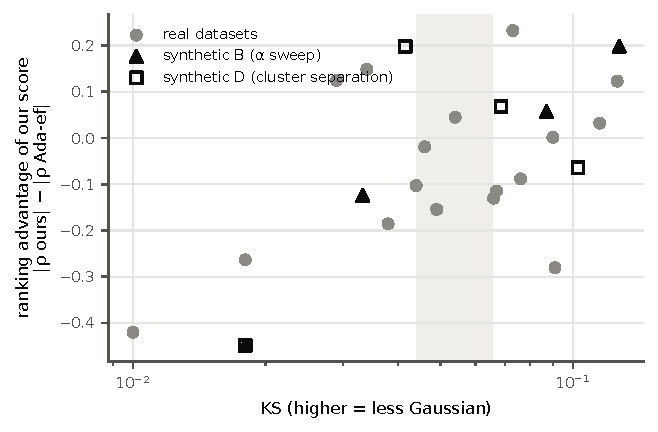
\includegraphics[width=\linewidth]{figures/fig4_controlled.pdf}
  \caption{Ranking advantage of the empirical score (its $|\rho|$ minus Ada-ef's) against KS, for the real datasets and for synthetic data with controlled anisotropy (B) and cluster
  separation (D).}
  \label{fig:controlled}
\end{figure}

\begin{figure}[h]
  \centering
  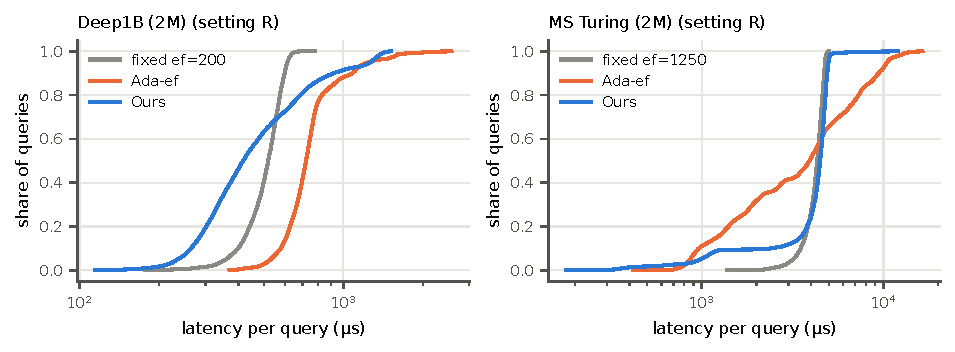
\includegraphics[width=\linewidth]{figures/fig3c_latency_cdf.pdf}
  \caption{Per-query latency on Deep1B and MS Turing (setting R). The empirical score spends less
  time on easy queries and more on hard ones; a fixed \ef{} spends about the same on all.}
  \label{fig:cdf}
\end{figure}

\begin{table*}[t]
  \caption{Time per distance computation, relative to fixed-\ef{} queries with the same distance count
  (settings P and R). Hard and easy: the 20\% of queries PercEF gives the largest and smallest \ef{},
  timed under the fixed \ef{} closest to PercEF's mean recall. Last column: PercEF's share of its
  distance computations spent on its hard queries.}
  \label{tab:querycost}
  \centering\footnotesize
  \resizebox{\linewidth}{!}{\begin{tabular}{llrrrrr}
\toprule
dataset & setting & KS & hard / fixed-ef time at same DC & easy / fixed-ef time at same DC & PercEF / fixed-ef time at same DC & PercEF DC on hard queries (\%) \\
\midrule
MS Turing (2M) & P & 0.010 & 1.009 & 1.003 & 0.991 & 95.1 \\
MS Turing (2M) & R & 0.010 & 1.003 & 0.997 & 0.981 & 97.9 \\
GloVe-100 & P & 0.018 & 1.036 & 0.803 & 1.025 & 95.7 \\
GloVe-100 & R & 0.018 & 1.036 & 0.803 & 1.014 & 97.3 \\
BIGANN (2M) & P & 0.029 & 1.076 & 0.807 & 1.032 & 50.5 \\
BIGANN (2M) & R & 0.029 & 1.087 & 0.800 & 1.025 & 39.0 \\
LAION-I2I & P & 0.034 & 1.191 & 0.842 & 1.043 & 58.0 \\
LAION-I2I & R & 0.034 & 1.174 & 0.809 & 1.057 & 54.3 \\
DBpedia-1536 & P & 0.038 & 1.048 & 0.885 & 1.000 & 81.2 \\
DBpedia-1536 & R & 0.038 & 1.057 & 0.834 & 1.036 & 66.1 \\
MS MARCO-384 & P & 0.044 & 1.132 & 0.816 & 1.004 & 30.4 \\
MS MARCO-384 & R & 0.044 & 1.134 & 0.827 & 0.971 & 30.8 \\
COCO-I2I & P & 0.046 & 1.148 & 0.925 & 1.053 & 43.8 \\
COCO-I2I & R & 0.046 & 1.168 & 0.908 & 1.051 & 35.9 \\
Cohere-1024 & P & 0.049 & 1.049 & 0.801 & 0.976 & 63.7 \\
Cohere-1024 & R & 0.049 & 1.066 & 0.837 & 1.027 & 71.2 \\
Yahoo-MiniLM & P & 0.054 & 1.084 & 0.890 & 1.022 & 44.9 \\
Yahoo-MiniLM & R & 0.054 & 1.088 & 0.893 & 1.029 & 39.8 \\
COCO-T2I & P & 0.056 & 1.005 & 1.005 & 1.011 & 100.0 \\
COCO-T2I & R & 0.056 & 1.001 & 1.001 & 1.014 & 100.0 \\
ImageNet-ALIGN & P & 0.058 & 1.009 & 1.009 & 1.031 & 100.0 \\
ImageNet-ALIGN & R & 0.058 & 1.000 & 1.000 & 1.027 & 100.0 \\
DeepImage-96 & P & 0.066 & 1.074 & 0.916 & 1.066 & 52.0 \\
DeepImage-96 & R & 0.066 & 1.089 & 0.910 & 1.076 & 43.6 \\
Deep1B (2M) & P & 0.067 & 1.092 & 0.889 & 1.053 & 34.4 \\
Deep1B (2M) & R & 0.067 & 1.084 & 0.882 & 1.074 & 43.9 \\
Fashion-MNIST & P & 0.073 & 1.093 & 0.980 & 1.017 & 30.3 \\
Fashion-MNIST & R & 0.073 & 1.091 & 0.978 & 1.015 & 25.6 \\
Landmark-DINO & P & 0.076 & 1.085 & 0.893 & 0.976 & 52.9 \\
Landmark-DINO & R & 0.076 & 1.090 & 0.892 & 0.997 & 49.0 \\
Yambda & P & 0.090 & 1.004 & 1.002 & 0.977 & 100.0 \\
Yambda & R & 0.090 & 0.999 & 0.978 & 0.989 & 100.0 \\
GIST-960 & P & 0.091 & 1.005 & 1.002 & 0.977 & 98.8 \\
GIST-960 & R & 0.091 & 1.005 & 1.002 & 0.981 & 99.4 \\
iNat-ResNet & P & 0.115 & 1.109 & 0.930 & 0.993 & 33.7 \\
iNat-ResNet & R & 0.115 & 1.123 & 0.912 & 1.000 & 30.0 \\
SIFT-1M & P & 0.126 & 1.050 & 0.896 & 1.005 & 42.7 \\
SIFT-1M & R & 0.126 & 1.060 & 0.894 & 1.006 & 28.9 \\
Last.fm & P & 0.216 & 0.999 & 0.999 & 0.985 & 100.0 \\
Last.fm & R & 0.216 & 0.996 & 0.996 & 0.994 & 100.0 \\
\bottomrule
\end{tabular}
}
\end{table*}

\clearpage
\end{document}
